\section{Neural Networks}


Neural networks, often at the heart of modern machine learning, have revolutionized numerous fields, from image and speech recognition to medical diagnosis and financial forecasting. Historically inspired by the structure and function of the brain, these computational models have evolved over the decades, both in complexity and capability. 

The term "neural network" was first coined in the mid-20th century, reflecting the initial goal of mimicking the human brain's intricate web of neurons and synapses. While modern neural networks have since diverged from strict biological replication, their foundational principles remain rooted in this early inspiration.

In this section, we aim to provide a comprehensive overview of neural networks, delving into their architecture, training mechanisms, and applications. We will also explore their significance in the realm of operations research and mathematical programming, emphasizing their optimization aspects and real-world applicability.

\subsection{Basic Concepts}

Neural networks, at their core, are composed of interconnected nodes or \textit{neurons}. These connections, often termed as \textit{weights}, play a pivotal role in the network's ability to learn and adapt. In this subsection, we will introduce the fundamental building blocks of neural networks.

\subsubsection{Neurons: Biological Inspiration and Mathematical Abstraction}

The concept of a neuron in artificial neural networks is inspired by biological neurons found in the brain. A biological neuron receives inputs through its dendrites, processes the information, and sends the output via its axon.

In the context of artificial neural networks, a neuron:
\begin{itemize}
    \item Receives multiple inputs.
    \item Multiplies each input by its associated weight.
    \item Sums the weighted inputs and adds a bias term.
    \item Passes the result through an activation function to produce an output.
\end{itemize}

Mathematically, the output \( y \) of a neuron can be represented as:
\[ y = f\left( \sum_{i} w_i x_i + b \right) \]
where \( w_i \) are the weights, \( x_i \) are the inputs, \( b \) is the bias, and \( f \) is the activation function.

\subsubsection{Activation Functions}

Activation functions introduce non-linearity into the network, enabling it to learn complex patterns. Some commonly used activation functions include:

\begin{itemize}
    \item \textbf{Sigmoid}: \( \sigma(z) = \frac{1}{1 + e^{-z}} \)
    \item \textbf{ReLU (Rectified Linear Unit)}: \( f(z) = \max(0, z) \)
    \item \textbf{Tanh}: \( f(z) = \tanh(z) \)
\end{itemize}

Each activation function has its own advantages and use-cases, depending on the specific problem and network architecture.

\subsubsection{Network Architecture}

A typical neural network consists of:
\begin{itemize}
    \item \textbf{Input Layer}: Represents the features of the data.
    \item \textbf{Hidden Layers}: One or more layers where the actual processing happens. Each layer contains multiple neurons.
    \item \textbf{Output Layer}: Produces the final prediction or classification result.
\end{itemize}

The depth (number of layers) and width (number of neurons in a layer) of a network can vary based on the complexity of the problem and the amount of data available.


\begin{figure}[h]
\centering
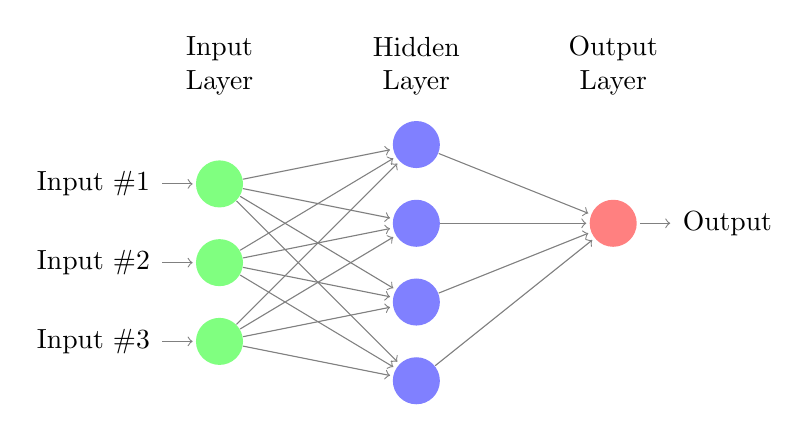
\begin{tikzpicture}[shorten >=1pt,->,draw=black!50, node distance=\layersep]
    \tikzstyle{every pin edge}=[<-,shorten <=1pt]
    \tikzstyle{neuron}=[circle,fill=black!25,minimum size=17pt,inner sep=0pt]
    \tikzstyle{input neuron}=[neuron, fill=green!50];
    \tikzstyle{output neuron}=[neuron, fill=red!50];
    \tikzstyle{hidden neuron}=[neuron, fill=blue!50];
    \tikzstyle{annot} = [text width=4em, text centered]

    % Define the separation between layers
    \def\layersep{2.5cm}

    % Draw the input layer nodes
    \foreach \name / \y in {1,...,3}
        \node[input neuron, pin=left:Input \#\y] (I-\name) at (0,-\y) {};

    % Draw the hidden layer nodes
    \foreach \name / \y in {1,...,4}
        \path[yshift=0.5cm]
            node[hidden neuron] (H-\name) at (\layersep,-\y cm) {};

    % Draw the output layer node
    \node[output neuron,pin={[pin edge={->}]right:Output}, right of=H-2] (O) {};

    % Connect every node in the input layer with every node in the hidden layer.
    \foreach \source in {1,...,3}
        \foreach \dest in {1,...,4}
            \path (I-\source) edge (H-\dest);

    % Connect every node in the hidden layer to the output layer
    \foreach \source in {1,...,4}
        \path (H-\source) edge (O);

    % Annotate the layers
    \node[annot,above of=H-1, node distance=1cm] (hl) {Hidden Layer};
    \node[annot,left of=hl] {Input Layer};
    \node[annot,right of=hl] {Output Layer};
\end{tikzpicture}
\caption{Basic architecture of a feedforward neural network.}
\end{figure}

\subsection{Feedforward Neural Networks}

Feedforward neural networks, often simply referred to as feedforward networks or multilayer perceptrons (MLPs), are the quintessential type of artificial neural network. As the name suggests, information in these networks flows in one direction: from the input layer, through any number of hidden layers, and finally to the output layer.

\subsubsection{Architecture}

A feedforward network consists of:
\begin{itemize}
    \item \textbf{Input Layer}: The initial layer where data is fed into the network. The number of neurons in this layer corresponds to the number of input features.
    \item \textbf{Hidden Layers}: These are intermediate layers between input and output. Each neuron in a hidden layer receives weighted inputs from the previous layer, processes it (typically with a nonlinear activation function), and sends its output to the next layer.
    \item \textbf{Output Layer}: The final layer that produces the network's prediction. The number of neurons here typically corresponds to the number of classes (for classification tasks) or to the desired output dimension (for regression tasks).
\end{itemize}

\subsubsection{Forward Propagation}

Forward propagation refers to the process of passing an input through the network to obtain an output. The steps are as follows:
\begin{enumerate}
    \item Provide the input data to the input layer.
    \item For each neuron in the first hidden layer, compute the weighted sum of its inputs and pass the result through its activation function.
    \item Repeat the above step for each subsequent hidden layer.
    \item In the output layer, compute the final output. For classification tasks, this often involves a softmax function to produce probability distributions over classes.
\end{enumerate}

Mathematically, for each layer \( l \) and neuron \( j \) in that layer, the output \( o_{l,j} \) is given by:
\[ o_{l,j} = f\left( \sum_{i} w_{l,i,j} o_{l-1,i} + b_{l,j} \right) \]
where \( w_{l,i,j} \) is the weight from neuron \( i \) in layer \( l-1 \) to neuron \( j \) in layer \( l \), \( b_{l,j} \) is the bias for neuron \( j \) in layer \( l \), and \( f \) is the activation function.

\subsubsection{Use Cases}

Feedforward networks are versatile and can be applied to a wide range of tasks, including:
\begin{itemize}
    \item \textbf{Regression}: Predicting a continuous value.
    \item \textbf{Classification}: Categorizing input data into predefined classes.
    \item \textbf{Function Approximation}: Learning a mapping from inputs to outputs.
    \item \textbf{Pattern Recognition}: Identifying patterns or regularities in data.
\end{itemize}

While feedforward networks are foundational and widely used, they have limitations, especially when dealing with sequential or spatial data. More specialized network architectures, such as recurrent or convolutional neural networks, are often preferred for such tasks.



\begin{figure}[h]
\centering
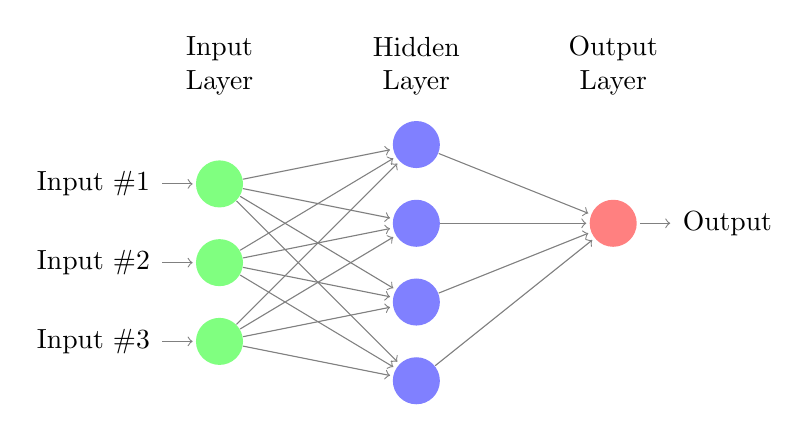
\begin{tikzpicture}[shorten >=1pt,->,draw=black!50, node distance=\layersep]
    \tikzstyle{every pin edge}=[<-,shorten <=1pt]
    \tikzstyle{neuron}=[circle,fill=black!25,minimum size=17pt,inner sep=0pt]
    \tikzstyle{input neuron}=[neuron, fill=green!50];
    \tikzstyle{output neuron}=[neuron, fill=red!50];
    \tikzstyle{hidden neuron}=[neuron, fill=blue!50];
    \tikzstyle{annot} = [text width=4em, text centered]

    % Define the separation between layers
    \def\layersep{2.5cm}

    % Draw the input layer nodes
    \foreach \name / \y in {1,...,3}
        \node[input neuron, pin=left:Input \#\y] (I-\name) at (0,-\y) {};

    % Draw the hidden layer nodes
    \foreach \name / \y in {1,...,4}
        \path[yshift=0.5cm]
            node[hidden neuron] (H-\name) at (\layersep,-\y cm) {};

    % Draw the output layer node
    \node[output neuron,pin={[pin edge={->}]right:Output}, right of=H-2] (O) {};

    % Connect every node in the input layer with every node in the hidden layer.
    \foreach \source in {1,...,3}
        \foreach \dest in {1,...,4}
            \path (I-\source) edge (H-\dest);

    % Connect every node in the hidden layer to the output layer
    \foreach \source in {1,...,4}
        \path (H-\source) edge (O);

    % Annotate the layers
    \node[annot,above of=H-1, node distance=1cm] (hl) {Hidden Layer};
    \node[annot,left of=hl] {Input Layer};
    \node[annot,right of=hl] {Output Layer};
\end{tikzpicture}
\caption{Architecture of a feedforward neural network.}
\end{figure}


\subsection{Training Neural Networks}

Training a neural network involves adjusting its weights and biases to minimize the difference between its predicted outputs and the actual target values. This process leverages optimization techniques to find the best possible parameters for the model.

\subsubsection{Loss Functions}

A loss function, or cost function, quantifies the difference between the predicted outputs and the actual target values. Commonly used loss functions include:
\begin{itemize}
    \item \textbf{Mean Squared Error (MSE)}: Used for regression tasks. It calculates the average of the squared differences between predictions and targets.
    \[ \text{MSE} = \frac{1}{n} \sum_{i=1}^{n} (y_i - \hat{y}_i)^2 \]
    where \( y_i \) is the actual value, \( \hat{y}_i \) is the predicted value, and \( n \) is the number of samples.
    
    \item \textbf{Cross-Entropy Loss}: Used for classification tasks. It measures the dissimilarity between the predicted probability distribution and the actual distribution.
    \[ \text{Cross-Entropy} = -\sum_{i=1}^{C} y_i \log(\hat{y}_i) \]
    where \( C \) is the number of classes, \( y_i \) is the actual probability of class \( i \), and \( \hat{y}_i \) is the predicted probability of class \( i \).
\end{itemize}

\subsubsection{Backpropagation}

Backpropagation is the cornerstone algorithm for training feedforward neural networks. It involves two main steps:
\begin{enumerate}
    \item \textbf{Forward Pass}: Input data is passed through the network to compute the predicted output.
    \item \textbf{Backward Pass}: The gradient of the loss function with respect to each weight is computed by the chain rule of calculus. These gradients are then used to update the weights in the direction that minimizes the loss.
\end{enumerate}

\subsubsection{Gradient Descent and Its Variants}

Gradient Descent is an optimization algorithm used to minimize the loss function. The basic idea is to adjust the weights in the direction of the steepest decrease in the loss. Variants of gradient descent include:
\begin{itemize}
    \item \textbf{Stochastic Gradient Descent (SGD)}: Updates the weights using only a single data point at each iteration.
    \item \textbf{Mini-Batch Gradient Descent}: Updates the weights using a subset (or batch) of the dataset at each iteration.
    \item \textbf{Momentum-Based Methods}: Incorporate a momentum term to accelerate convergence and overcome local minima.
\end{itemize}

\subsubsection{Regularization Techniques}

Regularization helps prevent overfitting, where the model performs well on the training data but poorly on unseen data. Common regularization techniques include:
\begin{itemize}
    \item \textbf{Dropout}: Randomly sets a fraction of the input units to 0 at each update during training, which helps prevent over-reliance on any single neuron.
    \item \textbf{L2 Regularization (Weight Decay)}: Adds a penalty to the loss function based on the magnitude of the weights, encouraging smaller weights.
\end{itemize}

In essence, training a neural network is an iterative process of adjusting weights and biases to minimize the loss, using optimization techniques and incorporating regularization to ensure generalization.

\subsection{Deep Learning}

Deep learning, a subset of machine learning, focuses on algorithms inspired by the structure and function of the brain called artificial neural networks. While traditional neural networks might contain a few hidden layers, deep learning networks can have dozens or even hundreds of layers. These deep networks are capable of discovering intricate structures in large datasets.

\subsubsection{Introduction to Deep Neural Networks}

Deep neural networks (DNNs) are neural networks with a significant number of layers. These networks aim to model high-level abstractions in data by using multiple processing layers, composed of multiple linear and non-linear transformations.

\subsubsection{Convolutional Neural Networks (CNNs)}

CNNs are a category of neural networks that have proven effective in areas such as image recognition and classification. They are designed to automatically and adaptively learn spatial hierarchies of features from input images.

\begin{itemize}
    \item \textbf{Convolutional Layer}: The core operation involves sliding a filter or kernel over the input data (such as an image) to produce a feature map or convolved feature.
    \item \textbf{Pooling Layer}: This layer periodically downsamples the spatial dimensions, reducing the computational complexity for upper layers.
    \item \textbf{Fully Connected Layer}: Neurons in a fully connected layer have connections to all activations in the previous layer, as seen in regular neural networks.
\end{itemize}

\subsubsection{Recurrent Neural Networks (RNNs)}

RNNs are designed to recognize patterns in sequences of data, such as text, genomes, handwriting, or the spoken word. Unlike traditional neural networks, RNNs have loops to allow information persistence.

\begin{itemize}
    \item \textbf{Long Short-Term Memory (LSTM)}: A special kind of RNN capable of learning long-term dependencies. LSTMs are explicitly designed to avoid long-term dependency issues, making them exceptionally well-suited for classifying, processing, and predicting time series and sequences with large time lags.
    \item \textbf{Gated Recurrent Units (GRU)}: A variant of LSTM, GRUs combine the forget and input gates into a single "update gate." They also merge the cell state and hidden state, resulting in a simpler model.
\end{itemize}

\subsubsection{Transfer Learning and Pre-trained Models}

Transfer learning is a machine learning method where a model developed for a task is reused as the starting point for a model on a second task. It's beneficial when dealing with datasets of limited size.

\begin{itemize}
    \item \textbf{Fine-tuning}: Adjusting the weights of a pre-trained model by continuing the backpropagation. It's used to adapt the neural network to the new task.
    \item \textbf{Feature Extraction}: Using representations learned by a previous network to extract meaningful features from new samples. A new classifier is then trained from scratch on top of the extracted features.
\end{itemize}

Deep learning, with its vast capabilities and applications, has been at the forefront of the AI revolution, driving advancements in various domains and setting new benchmarks in numerous tasks.

\subsection{Optimization in Neural Networks}

Optimization plays a pivotal role in the training of neural networks. The primary goal is to adjust the model's parameters to minimize the loss function, which measures the difference between the predicted outputs and the actual target values. This section delves into the challenges and techniques associated with optimization in neural networks.

\subsubsection{Challenges in Neural Network Optimization}

Training neural networks presents several optimization challenges:

\begin{itemize}
    \item \textbf{Non-Convexity}: Unlike convex optimization problems, neural network optimization landscapes are riddled with local minima, saddle points, and flat regions. This makes it challenging to find the global minimum.
    \item \textbf{Vanishing and Exploding Gradients}: Deep networks often suffer from gradients that become too small (vanish) or too large (explode) as they are propagated backward through the layers. This can severely hamper convergence.
    \item \textbf{Plateaus}: Regions where the gradient is near zero, making the optimization process slow.
    \item \textbf{Overfitting}: A model with too many parameters might fit the training data perfectly but perform poorly on unseen data.
\end{itemize}

\subsubsection{Advanced Optimization Techniques}

To address the challenges of neural network optimization, several advanced techniques have been developed:

\begin{itemize}
    \item \textbf{Adam}: Combines the benefits of two other extensions of stochastic gradient descent: AdaGrad and RMSProp. Adam computes adaptive learning rates for each parameter and uses moving averages of the parameters.
    \item \textbf{RMSprop}: Modifies SGD to use a moving average of the squared gradient to normalize the gradient itself.
    \item \textbf{Momentum}: Adds a fraction of the update vector from the past time step to the current update vector. It helps in accelerating SGD in the relevant direction and dampens oscillations.
    \item \textbf{Learning Rate Scheduling}: Gradually decreasing the learning rate during training can lead to better convergence. Common strategies include step decay, exponential decay, and 1/t decay.
\end{itemize}

\subsubsection{Hyperparameter Tuning}

Hyperparameters, parameters not learned from the training process, play a crucial role in the performance of neural networks. Efficiently tuning these can significantly improve a model's performance. Common techniques include:

\begin{itemize}
    \item \textbf{Grid Search}: Exhaustively tries every combination of hyperparameters.
    \item \textbf{Random Search}: Randomly samples the space of hyperparameters.
    \item \textbf{Bayesian Optimization}: Uses probability to find the minimum of a function. It builds a probabilistic model of the function and uses it to select the most promising hyperparameters to evaluate in the true objective function.
\end{itemize}

Optimization in neural networks is a vast and active area of research. As models grow in complexity and are applied to an ever-expanding set of tasks, the tools and techniques for optimization continue to evolve.

\subsection{Regularization and Generalization}

In the context of neural networks, regularization refers to techniques that prevent overfitting, ensuring that the model generalizes well to unseen data. Overfitting occurs when a model learns the training data too closely, including its noise and outliers, leading to poor performance on new, unseen data. This section explores various regularization techniques and their importance in enhancing model generalization.

\subsubsection{Overfitting and Underfitting}

Understanding the balance between overfitting and underfitting is crucial:

\begin{itemize}
    \item \textbf{Overfitting}: The model performs exceptionally well on the training data but poorly on the validation or test data. This indicates that the model has learned the training data's noise and outliers.
    \item \textbf{Underfitting}: The model performs poorly on both the training and validation/test data. This suggests that the model is too simple to capture the underlying patterns in the data.
\end{itemize}

\subsubsection{Techniques for Regularization}

Several techniques can be employed to prevent overfitting and enhance generalization:

\begin{itemize}
    \item \textbf{L1 and L2 Regularization}: These techniques add a penalty to the loss function based on the magnitude of the weights. L1 regularization adds a penalty proportional to the absolute value of the weights, leading to sparsity, while L2 regularization adds a penalty proportional to the square of the weights.
    \item \textbf{Dropout}: During training, random subsets of neurons are "dropped out" or temporarily deactivated. This prevents any single neuron from becoming overly specialized.
    \item \textbf{Early Stopping}: Training is halted once the performance on a validation set stops improving, even if the performance on the training set continues to improve.
    \item \textbf{Data Augmentation}: By artificially increasing the size of the training set using transformations like rotations, translations, and zooms, the model becomes more robust and less likely to overfit.
    \item \textbf{Batch Normalization}: Normalizes the activations of each layer to maintain a mean close to 0 and a standard deviation close to 1. This can improve generalization and also allows for faster training.
\end{itemize}

\subsubsection{Model Evaluation}

Ensuring that a model generalizes well requires proper evaluation:

\begin{itemize}
    \item \textbf{Training, Validation, and Test Splits}: Data is divided into three sets. The training set is used to train the model, the validation set is used to tune hyperparameters and prevent overfitting, and the test set is used to evaluate the model's final performance.
    \item \textbf{Cross-Validation}: The training set is divided into \( k \) subsets. The model is trained \( k \) times, each time using \( k-1 \) subsets for training and the remaining subset for validation. The results are then averaged to produce a more robust performance metric.
\end{itemize}

Regularization and generalization are essential aspects of neural network training. Properly regularized models are more likely to perform well in real-world scenarios, making them more valuable and reliable in practical applications.

\subsection{Applications in Operations Research}

Operations Research (OR) focuses on the application of analytical methods to aid decision-making. With the rise of neural networks and deep learning, there has been a convergence between OR and machine learning, leading to enhanced models and solutions for complex problems. This section delves into the intersection of neural networks and OR, highlighting key applications.

\subsubsection{Neural Networks in Forecasting}

Forecasting is a cornerstone of OR, especially in areas like supply chain management, finance, and production planning. Neural networks, with their ability to model non-linear relationships and handle large datasets, have become valuable tools for:

\begin{itemize}
    \item \textbf{Demand Forecasting}: Predicting future product demand to optimize inventory levels.
    \item \textbf{Financial Forecasting}: Predicting stock prices, currency exchange rates, and other financial metrics.
    \item \textbf{Energy Consumption Forecasting}: Estimating future energy needs for efficient grid management.
\end{itemize}

\subsubsection{Combinatorial Optimization using Neural Networks}

Combinatorial optimization problems, such as the traveling salesman problem or the knapsack problem, are NP-hard. Neural networks, especially recurrent networks, have been explored as heuristic solvers:

\begin{itemize}
    \item \textbf{Hopfield Networks}: Used for optimization problems by finding low-energy states that correspond to good solutions.
    \item \textbf{Pointer Networks}: A type of recurrent neural network designed to predict a permutation of the input, suitable for sequence-to-sequence problems.
\end{itemize}

\subsubsection{Reinforcement Learning and Neural Networks in Decision-Making}

Reinforcement learning (RL), combined with deep neural networks (often termed Deep RL), has shown promise in decision-making tasks in OR:

\begin{itemize}
    \item \textbf{Inventory Management}: Using RL to determine optimal ordering policies in dynamic environments.
    \item \textbf{Dynamic Pricing}: Adjusting prices in real-time based on demand, competition, and other factors.
    \item \textbf{Supply Chain Optimization}: End-to-end optimization of supply chains using RL to make sequential decisions.
\end{itemize}

\subsubsection{Case Studies}

To provide practical insights, it's beneficial to delve into real-world applications where neural networks have enhanced OR methodologies:

\begin{itemize}
    \item \textbf{Airline Revenue Management}: Using neural networks to predict booking patterns and optimize seat allocations.
    \item \textbf{Manufacturing Quality Control}: Implementing convolutional neural networks (CNNs) for visual inspection and defect detection.
    \item \textbf{Transportation and Route Planning}: Leveraging recurrent networks to predict traffic patterns and optimize route schedules.
\end{itemize}

The synergy between neural networks and operations research has opened avenues for innovative solutions, pushing the boundaries of what's achievable in decision science.

\subsection{Future Trends and Challenges}

As neural networks continue to evolve and permeate various domains, it's essential to understand the emerging trends and challenges that will shape the next era of neural network research and application. This section provides insights into what the future might hold and the hurdles that need to be addressed.

\subsubsection{Emerging Trends}

Several trends are gaining momentum in the realm of neural networks:

\begin{itemize}
    \item \textbf{Neural Architecture Search (NAS)}: Automated methods for finding the best network architecture, eliminating much of the manual trial and error.
    \item \textbf{Self-Supervised Learning}: Training models using data that is labeled by the model itself, reducing the need for extensive labeled datasets.
    \item \textbf{Neural Networks in Edge Devices}: With the rise of IoT, there's a push towards running neural networks on edge devices (like smartphones and sensors) rather than centralized servers.
    \item \textbf{Quantum Neural Networks}: Exploring the intersection of quantum computing and neural networks, aiming to harness the computational power of quantum systems.
\end{itemize}

\subsubsection{Challenges Ahead}

While the potential of neural networks is vast, several challenges need to be addressed:

\begin{itemize}
    \item \textbf{Explainability and Interpretability}: As neural networks become more complex, understanding their decision-making processes becomes crucial, especially in sensitive areas like healthcare and finance.
    \item \textbf{Robustness and Security}: Ensuring that neural networks are resistant to adversarial attacks and can operate reliably in diverse conditions.
    \item \textbf{Ethical Considerations}: Addressing biases in neural network predictions and ensuring that their applications respect privacy and ethical standards.
    \item \textbf{Environmental Concerns}: Training large neural networks requires significant computational resources, leading to concerns about their carbon footprint.
\end{itemize}

\subsubsection{Collaborative and Multi-modal Learning}

The future might see more integration of different data sources and types:

\begin{itemize}
    \item \textbf{Fusion of Modalities}: Combining data from different sources (like images, text, and sound) to improve prediction accuracy.
    \item \textbf{Collaborative Learning}: Multiple neural network models collaborating to solve a task, leveraging their individual strengths.
\end{itemize}

\subsubsection{Continual and Lifelong Learning}

As the real world is dynamic, there's a growing interest in models that can learn continuously:

\begin{itemize}
    \item \textbf{Adaptation to New Data}: Models that can update their knowledge without forgetting previously learned information.
    \item \textbf{Task Agnostic Learning}: Models that can learn to perform new tasks using minimal data.
\end{itemize}

The landscape of neural networks is ever-evolving, with each advancement bringing new opportunities and challenges. By staying informed and adaptive, researchers and practitioners can harness the full potential of neural networks in diverse applications.

\subsection{Conclusion and Outlook}

Neural networks have undeniably revolutionized the field of machine learning, offering powerful tools to model complex patterns and relationships in data. From their foundational architectures to their advanced applications in operations research, they have demonstrated versatility and potential across numerous domains.

\subsubsection{Recapitulation}

We began our exploration with the foundational concepts, understanding the architecture and mechanics of feedforward networks. As we delved deeper, the complexities of training, the challenges of optimization, and the nuances of regularization became evident. The convergence of operations research and neural networks showcased the interdisciplinary nature of modern computational challenges. Furthermore, the future trends highlighted the rapid pace of innovation in this domain, with emerging techniques and paradigms poised to shape the next generation of neural network applications.

\subsubsection{The Road Ahead}

While the achievements in neural network research and application are commendable, the journey is far from over. The challenges of explainability, robustness, and ethical considerations underscore the broader implications of widespread neural network deployment. As we move towards an era dominated by AI and machine learning, the role of neural networks will be pivotal.

\begin{itemize}
    \item \textbf{Interdisciplinary Collaboration}: The fusion of knowledge from diverse fields, such as neuroscience, quantum physics, and social sciences, can offer fresh perspectives and breakthroughs.
    \item \textbf{Sustainable AI}: Addressing the environmental impact of large-scale neural network training will be crucial. Efficient algorithms, hardware optimization, and green energy sources can mitigate the carbon footprint.
    \item \textbf{Human-AI Symbiosis}: Instead of viewing AI as a replacement, the future might see more collaborative efforts where humans and AI systems work in tandem, leveraging their respective strengths.
\end{itemize}

\subsubsection{Final Thoughts}

Neural networks, as a reflection of our quest to understand and replicate human intelligence, are a testament to human ingenuity. As we stand on the cusp of new discoveries and innovations, it's essential to approach the future with a blend of optimism, caution, and curiosity. The potential of neural networks is vast, but so is the responsibility that accompanies their application.

\subsection{Further Reading and Resources}

For those eager to delve deeper into the intricacies of neural networks and their applications, this section provides a curated list of resources, ranging from foundational texts to cutting-edge research papers.

\subsubsection{Foundational Texts}

\begin{itemize}
    \item \textit{Neural Networks and Deep Learning} by Michael Nielsen: An interactive online textbook offering a deep dive into the basics of neural networks.
    \item \textit{Deep Learning} by Ian Goodfellow, Yoshua Bengio, and Aaron Courville: A comprehensive text covering a wide range of topics in deep learning.
    \item \textit{Pattern Recognition and Machine Learning} by Christopher M. Bishop: A foundational text that covers neural networks within the broader context of machine learning.
\end{itemize}

\subsubsection{Online Courses and Tutorials}

\begin{itemize}
    \item \textbf{Coursera's Deep Learning Specialization} by Andrew Ng: A series of courses that provide a thorough introduction to deep learning, neural networks, and their applications.
    \item \textbf{Neural Networks for Machine Learning} on Coursera by Geoffrey Hinton: A course that delves into the theory and practice of neural networks.
    \item \textbf{TensorFlow Tutorials}: Official tutorials for TensorFlow, a popular deep learning framework, covering a wide range of topics and applications.
\end{itemize}

\subsubsection{Research Journals and Conferences}

\begin{itemize}
    \item \textbf{Journal of Artificial Neural Networks}: A peer-reviewed journal dedicated to the latest advancements in neural network research.
    \item \textbf{NeurIPS (Conference on Neural Information Processing Systems)}: One of the premier conferences in the field, showcasing cutting-edge research and developments.
    \item \textbf{ICLR (International Conference on Learning Representations)}: A conference focusing on representation learning and deep learning.
\end{itemize}

\subsubsection{Online Communities and Forums}

\begin{itemize}
    \item \textbf{arXiv}: A preprint server where researchers share their latest findings before formal peer review. The \textit{cs.LG} (Learning) category often features neural network research.
    \item \textbf{Reddit's r/MachineLearning}: A community where researchers, practitioners, and enthusiasts discuss the latest in machine learning and neural networks.
    \item \textbf{Stack Exchange's Cross Validated}: A Q\&A forum for statistics, machine learning, data analysis, and related topics.
\end{itemize}

As the field of neural networks continues to evolve, staying updated with the latest research, tools, and methodologies is crucial. These resources provide a starting point, but the journey of exploration and learning is endless.

\subsection{Glossary of Terms}

To aid in understanding and referencing, this section provides a concise glossary of key terms and concepts discussed throughout the book.

\begin{description}
    \item[Activation Function:] A mathematical function applied to a neuron's output, introducing non-linearity to the model. Common examples include the sigmoid, tanh, and ReLU functions.
    
    \item[Backpropagation:] The primary algorithm for training feedforward neural networks, involving the propagation of the error backward through the network to update weights.
    
    \item[Convolutional Neural Network (CNN):] A type of deep learning model primarily used for image processing tasks, characterized by its convolutional layers.
    
    \item[Deep Learning:] A subset of machine learning focused on algorithms inspired by the structure and function of the brain, primarily neural networks with three or more layers.
    
    \item[Epoch:] One complete forward and backward pass of all training samples during the training process.
    
    \item[Feedforward Neural Network:] A type of neural network where connections between nodes do not form cycles.
    
    \item[Gradient Descent:] An optimization algorithm used to minimize the loss function by iteratively adjusting model parameters.
    
    \item[Hidden Layer:] Layers in a neural network that are neither input nor output layers.
    
    \item[Learning Rate:] A hyperparameter that determines the step size during gradient descent optimization.
    
    \item[Loss Function:] A mathematical function that quantifies the difference between the predicted output and the actual output. Common examples include Mean Squared Error (MSE) and Cross-Entropy Loss.
    
    \item[Neuron:] The basic unit of computation in a neural network, often called a node or unit.
    
    \item[Overfitting:] A modeling error that occurs when a machine learning model captures noise in the training data and performs poorly on unseen data.
    
    \item[Recurrent Neural Network (RNN):] A type of neural network designed to recognize patterns in sequences of data by maintaining a memory of previous inputs.
    
    \item[Regularization:] Techniques used to prevent overfitting in a neural network, such as L1/L2 regularization and dropout.
    
    \item[Transfer Learning:] A machine learning method where a pre-trained model is fine-tuned for a different but related task.
    
    \item[Weight:] A parameter within a neural network that transforms input data within the network's layers.
\end{description}

This glossary serves as a quick reference guide, ensuring clarity and understanding of the fundamental concepts in neural networks. As the field continues to evolve, new terms and concepts will emerge, enriching the lexicon of this exciting domain.

\begin{resource}
See \url{http://citeseerx.ist.psu.edu/viewdoc/download;jsessionid=4982C26EC5F25564BCC239FD3785E2D3?doi=10.1.1.210.3547&rep=rep1&type=pdf} for many other helpful tips on using \ipopt.
\end{resource}
